%%%%%%%%%%%%%%%%%%%%%%%%%%%%%%%%%%%%%%%%% Preamble %%%%%%%%%%%%%%%%%%%%%%%%%%%%%%%%%%%%%%%%%

\documentclass[12pt]{report}

\usepackage{titling} % makes following commands available
\title{Catalytic properties at the nanoscale probed by surface X-ray diffraction and coherent diffraction imaging}
\author{David Simonne}
\date{\today}

%%%%%%%%%%%%%%%%%%%%%%%%%%%%%%%%%%%%%%%%%% Colours %%%%%%%%%%%%%%%%%%%%%%%%%%%%%%%%%%%%%%%%%%

\usepackage{xcolor}

\definecolor{ArgonColor}{HTML}{008FD5}
\definecolor{AmmoniaColor}{HTML}{DD65B0}
\definecolor{OxygenColor}{HTML}{FC4F30}
\definecolor{NitrogenColor}{HTML}{810F7C}
\definecolor{NitrousOxideColor}{HTML}{8B8B8B}
\definecolor{NitrogenOxideColor}{HTML}{6D904F}
\definecolor{WaterColor}{HTML}{E5AE38}

\definecolor{Ostwald}{HTML}{800080}
\definecolor{Haber}{HTML}{158466}

\definecolor{LightBlue}{RGB}{30,75,180}
\definecolor{LUBlue}{RGB}{0,0,128}
\definecolor{LUGrey}{RGB}{77,76,68}
\definecolor{Prune}{RGB}{99,0,60}
\definecolor{Important}{HTML}{980000}

\definecolor{DarkFern}{HTML}{407428}
\definecolor{DarkCharcoal}{HTML}{4D4944}
\definecolor{DarkBlue}{HTML}{23373B}
\definecolor{DarkOrange}{HTML}{EA7500}
\definecolor{LightOrange}{HTML}{F9D6B3}
\definecolor{Blue}{HTML}{13406a}

\colorlet{lightblue}{blue!60}
\colorlet{lightorange}{orange!60}
\colorlet{lightgreen}{green!60}
\colorlet{lightred}{red!60}
\colorlet{lightgray}{gray!60}
\colorlet{lightbrown}{brown!60}
\colorlet{lightpink}{pink!60}
\colorlet{lightviolet}{violet!60}

\colorlet{shadecolor}{gray!40}

%%%%%%%%%%%%%%%%%%%%%%%%%%%%%%%%%%%%%%%% Page layout %%%%%%%%%%%%%%%%%%%%%%%%%%%%%%%%%%%%%%%%

\usepackage[
    a4paper,
    width=155mm,
    headheight=110pt,
    top=25mm,
    bottom=25mm
]{geometry}

\usepackage{etoolbox} % Apply different styles
\usepackage{fancyhdr}
\pagestyle{fancy}
\renewcommand{\chaptermark}[1]{\markboth{#1}{}}
\renewcommand{\sectionmark}[1]{\markright{\thesection\ #1}}

\fancypagestyle{main}{% Define fancy style for thesis
    \fancyhead[L]{\chaptername \, \thechapter:  \small{\textsf{\leftmark}}}
    \fancyhead[R]{\small{\textsf{\rightmark}}}
    \fancyfoot[R]{\small{\thepage}}
    \fancyfoot[L]{\small{\theauthor}}
    \fancyfoot[C]{}
    \renewcommand{\headrulewidth}{0.4pt}%
    \renewcommand{\footrulewidth}{0.4pt}%
}
\appto\mainmatter{\pagestyle{main}}

\fancypagestyle{plain}{% Define plain style for table of contents and acknowledgements
    \fancyhf{}
    \fancyfoot[C]{\thepage}
    \renewcommand{\headrulewidth}{0pt}%
    \renewcommand{\footrulewidth}{0.4pt}%
}
\appto\frontmatter{\pagestyle{plain}}

\usepackage{sectsty} % To colour sections, raise an error on underbar
\chapterfont{\color{Prune}}
\sectionfont{\color{LUGrey}}
\subsectionfont{\color{LUGrey}}
\subsubsectionfont{\color{LUGrey}}

%%%%%%%%%%%%%%%%%%%%%%%%%%%%%%%%%%%%%%%%%% Citation %%%%%%%%%%%%%%%%%%%%%%%%%%%%%%%%%%%%%%%%%%

\usepackage[style=authoryear,sorting=none]{biblatex}
%    nty Sort by name, title, year.
%    nyt Sort by name, year, title.
%    nyvt Sort by name, year, volume, title.
%    anyt Sort by alphabetic label, name, year, title.
%    anyvt Sort by alphabetic label, name, year, volume, title.
%    ynt Sort by year, name, title.
%    ydnt Sort by year (descending), name, title.
%    none Do not sort at all. All entries are processed in citation order.
\addbibresource{/home/david/Documents/PhD/PhdThesis/references.bib}

%%%%%%%%%%%%%%%%%%%%%%%%%%%%%%%%%%%%%%% Other packages %%%%%%%%%%%%%%%%%%%%%%%%%%%%%%%%%%%%%%%

\usepackage[utf8]{inputenc} % Use accents in source code
\usepackage[T1]{fontenc} % Show accents in output

\usepackage{lipsum} % Latin blabla
\usepackage{lmodern} % to avoid errors in font size
\usepackage[british]{babel}
\usepackage{setspace} % Space between lines
\usepackage{mathtools}
\usepackage{tikz} % Drawing
\usetikzlibrary{shapes.geometric, arrows, positioning, calc}
\usepackage{colortbl} % Colour the lines in the tables
\usepackage{minted} % Format code
\usepackage[version=4]{mhchem}
\usepackage{animate} % for animations in 3D

\usepackage{textcomp} % To avoid warnings in gensymb
\usepackage{gensymb} % for degree symbol

\usepackage{siunitx} % Units
\DeclareSIUnit\angstrom{\text {Å}}

\usepackage{graphicx} % Insert images
\graphicspath{{/home/david/Documents/PhD/Figures/}}

\usepackage[hypcap=true,font={small,it},justification=centering]{caption}
\captionsetup{belowskip=2pt,aboveskip=2pt}

\usepackage{scrextend} % Forcer la 4eme  de couverture en page pair
\usepackage{mdframed} % Entourer un paragraphe
\usepackage{multirow} % Mettre un texte sur plusieurs rangées
\usepackage{multicol} % Mettre un texte sur plusieurs colonnes
\usepackage{array} % Create tables as arrays
\usepackage{csquotes}
\usepackage{booktabs} % for \midrule and such

\usepackage[
    colorlinks = true,
    linkcolor = LightBlue,
    urlcolor  = LightBlue,
    citecolor = LightBlue,
    anchorcolor = LightBlue,
]{hyperref} % load last to avoid errors

%%%%%%%%%%%%%%%%%%%%%%%%%%%%%%%%%%%%%%%%%% Commands %%%%%%%%%%%%%%%%%%%%%%%%%%%%%%%%%%%%%%%%%

\newcommand{\argon}{{\textcolor{ArgonColor}{\ce{Ar}\,}}}
\newcommand{\ammonia}{{\textcolor{AmmoniaColor}{\ce{NH_3}\,}}}
\newcommand{\nitrousoxide}{{\textcolor{NitrousOxideColor}{\ce{N_2O}\,}}}
\newcommand{\water}{{\textcolor{WaterColor}{\ce{H_2O}\,}}}
\newcommand{\nitrogen}{{\textcolor{NitrogenColor}{\ce{N_2}\,}}}
\newcommand{\nitricacid}{{\textcolor{DarkOrange}{\ce{HNO_3}\,}}}
\newcommand{\nitricoxide}{{\textcolor{NitrogenOxideColor}{\ce{NO}\,}}}
\newcommand{\dioxygen}{{\textcolor{OxygenColor}{\ce{O_2}\,}}}
\newcommand{\ptthreeofour}{{\textcolor{Important}{Pt$_3$O$_4$\,}}}
\newcommand{\ammoniumnitrate}{{\textcolor{Blue}{\ce{NH_4NO_3}\,}}}

\newcommand{\yes}{{\textcolor{green}{0}}}

\newcommand{\no}{{\textcolor{red}{x}}}
\newcommand{\ra}[1]{\renewcommand{\arraystretch}{#1}}

%%%%%%%%%%%%%%%%%%%%%%%%%%%%%%%%%%%%%%%%%% Document %%%%%%%%%%%%%%%%%%%%%%%%%%%%%%%%%%%%%%%%%%

\begin{document}

% Title page
    \begin{titlepage}

\newgeometry{left=6cm,bottom=1cm, top=1cm, right=1cm}

\tikz[remember picture,overlay] \node[opacity=1,inner sep=0pt] at (-13mm,-135mm){
\includegraphics{logo/Bandeau_UPaS.pdf}};

% fonte sans empattement pour la page de titre
\fontfamily{fvs}\fontseries{m}\selectfont

%*****************************************************
%******** NUMÉRO D'ORDRE DE LA THÈSE À COMPLÉTER *****
%******** POUR LE SECOND DÉPOT                   *****
%*****************************************************

\color{white}

\begin{picture}(0,0)

\put(-110,-743){\rotatebox{90}{NNT: 2020UPASA000}}
\end{picture}

\vspace{-12mm}
\flushright \includegraphics[height=2.1cm]{logo/CEA.png} \hspace{7mm}
\includegraphics[height=2.1cm]{logo/SOLEIL.png}

%*****************************************************
%******************** TITRE **************************
%*****************************************************

\flushright
\vspace{10mm}
\color{Prune}
\fontfamily{cmss}\fontseries{m}\fontsize{22}{26}\selectfont
Propriétés catalytiques à l'échelle nanométrique sondées par diffraction des rayons X de surface et imagerie de  diffraction cohérente.

\normalsize
\color{black}
\Large{\textit{Catalytic properties at the nanoscale probed by surface x-ray diffraction and coherent diffraction imaging}}
%*****************************************************

\vspace{1.5cm}
\normalsize
\textbf{Thèse de doctorat de l'Université Paris-Saclay}

\vspace{15mm}

École doctorale n$^{\circ}$ 000, dénomination et sigle\\
\small Spécialité de doctorat: Physique\\
\footnotesize Unité de recherche: voir annexe\\
\footnotesize Référent: : voir annexe\\
\vspace{15mm}

\textbf{Thèse présentée et soutenue à .....,\\ le .... 2023, par}\\
\bigskip
\Large {\color{Prune} \textbf{David SIMONNE}}

%************************************
\vspace{\fill} % ALIGNER LE TABLEAU EN BAS DE PAGE
%************************************

\bigskip
\flushleft
\scriptsize
\begin{tabular}{|p{7cm}l}
\arrayrulecolor{Prune}
{\footnotesize \textbf{Composition du jury}}\\
& \\
\textbf{Prénom Nom} &   Président/e\\ 
Titre, Affiliation & \\
\textbf{Prénom Nom} &  Rapportrice \\ 
Titre, Affiliation   &   \\ 
\textbf{Prénom Nom} &  Rapporteur \\ 
Titre, Affiliation  &   \\ 
\textbf{Prénom Nom} &  Examinatrice \\ 
Titre, Affiliation   &   \\ 
\textbf{Prénom Nom} &  Examinateur \\ 
Titre, Affiliation   &   \\ 
\textbf{Prénom Nom} &  Examinateur \\ 
Titre, Affiliationt   &   \\ 

\end{tabular} 

\medskip
\begin{tabular}{|p{7cm}l}
\arrayrulecolor{Prune}
{\footnotesize \textbf{Direction de la thèse}}\\
& \\
\textbf{Alessandro Coati} & Directeur\\
Dr., Synchrotron SOLEIL & \\
\textbf{Andrea Resta} & Codirecteur\\
Dr., Synchrotron SOLEIL & \\
\textbf{Marie-Ingrid Richard} & Coencadrante\\
Dr., CEA Grenoble & \\

\end{tabular} 

\end{titlepage}

% Optional Chapters
    %\chapter*{Dedication}
    %\chapter*{Declaration}
    \chapter*{Acknowledgements}
    I extend my deepest gratitude to Andrea for his unwavering support throughout the duration of this thesis.
You have contaminated me with your love of Linux and open source technology, and set a strong example in terms of commuting to work by bicycle, which I failed to follow in rainy and cold days.
Thank you very much for all the feedback that you gave me about this thesis, down to the details in the figure placement, fontsize or linewidth, and sentence length.
Pursuing your interest in the study of the ammonia oxidation has allowed me to explore a large subject.
This work has given me a sense of purpose, as it feels like my contribution is ever so slightly adding to the global endeavor in combating global warming and climate change.

I am immensely grateful for the shared beamtimes, the camaraderie during strenuous long shifts in summer or winter, skipping breakfast or dinner, compiling data while monitoring the sample heater.

Thank you Alessandro for being engaged in everything you do, at work and outside, for taking care of all the tedious work so that I could have the best possible experience, for inviting me to have meals and sometimes bringing me home after work, and for providing the SixS beamline with good italian coffee.

Thank you Marie-Ingrid for being so driven by your love of science that everybody around wants to participate, for arranging my stay in Grenoble and bringing all of the padawans to conferences, for always being in a good mood and ready to discuss new challenging experiments.

Thank you to my three advisors for being good mentors, allowing me to teach, to participate in schools and numerous beamtimes, for having my best interest in mind at all times and for trusting me.
I have learned an incredible amount from each of you and particularly appreciated the beamtime at Diamond, during which the four of us collected many electrons, but also shared meaningful conversations around a pint of beer and delicious stew.

I am very grateful to the research staff of SixS, to Alina and Yves for helping me when I was lost in the reciprocal space, to Benjamin without which none of the experiments could be possible, and to Michèle for her numerous advices.
Thank you also Frédéric for spending a lot of time in helping us regarding BCDI and SXRD code development.
Thank you to all the young researchers at SOLEIL for creating a group so that Saclay did not feel too remote and secluded.

I of course have a specific thought for the Grenoble legions, half of whom I don't know half as well as I should like, and half of which I know from half my life spent in beamtime.
Maxime, for introducing me to the world of political satire videos during ammonia oxidation cycles at SixS; Corentin, for the delightful culinary explorations in Grenoble, and for lending me the ID01 bicycle; Clément, for your constant positivity and our conversations about the promising future of PhD students; Nikita and Mattia, for the shared moments over a refreshing beer and the intense MSSBB games during Hercules; Ewen, for representing Bretagne alongside me; Edoardo, for the initiative of LAN parties, and the unforgettable Quake games; and Noor, for being an exceptional office (and coffee) mate in Grenoble.

I would also like to thank Steven for his good advice and for kind conversations, as well as Tobias and Joël for facilitating my stay in Grenoble for a few months during this thesis.
Thank you Vincent for letting me participate in the engaging ESRF tutorials, and Jérôme for starting the large work of bringing our BCDI community together in code development.
My heartfelt appreciation to Sarah and Stéphane for their warm hospitality in Marseille and their engaging discussions.

I feel very grateful towards Virginie and Christian who have followed me during the thesis by participating in the CSI, even available on weekends so that I would not miss registrations deadlines.

Thank you Andrea, Davide, Elisa and all the others from the university of Torino for making me want to pursue an academic path.
Thank you Davide again for hosting me in Grenoble after the ESRF user meeting because my train got cancelled, thank you Alessia and Giorgio for welcoming me.

Thank you to all the MaMaSELF members without which I would never have kept studiying physics and material science, and thus missed on studying in many countries, discovering new cultures, and mindsets.
Thank you Michael for bringing me to the world of neutron diffraction at Munich, and for letting me participate in my first beamtime at the ILL with Ulrike, a master and PhD student that had to learn a lot fast, but sadly not fast enough to handle the beam polarisation well.

Thank you to all the professors from Rennes that transmitted me their love of physics, especially Pr. Guérin that permitted me to study one year in Japan, thank you to Pr. Iwai for accepting me as part of his group in Sendaï.

Finally, to my family, whose unwavering support has bolstered my every endeavor, to Lucas, whose shared passion for science has been a source of motivation, and to my parents, for their trust and encouragement in my global pursuits.
Thank you to all my friends that have seen me being projected in numerous states during those three years, and without which I would probably not have kept the same level of sanity.

I extend my thanks to the esteemed members of the jury for their invaluable feedback and constructive critique, shaping the course of this work.

Furthermore, I acknowledge the invaluable support and resources provided by synchrotron SOLEIL, the CEA, and the ERC Carine, without which this research endeavor would not have been feasible.

Lastly, I express my gratitude to all those who have, in various capacities, contributed to the completion of this thesis.

\newpage

\frontmatter
% Table of contents, list of figures, and list of tables
{\hypersetup{linkcolor=black}
    \tableofcontents
    \listoffigures
    \listoftables
}

\mainmatter
% Introduction
    \chapter{Introduction} 
    \textcolor{red}{(The Introduction chapter should contain background information as appropriate, plus definitions of all special and general terms. Your topic should be: clearly stated and defined; have a clear overall purpose; and have clear, relevant and coherent aims and objectives. It is also informative to give a brief description of the contents of the remaining chapters of the thesis. This alerts the reader and prepares them for the rest of the thesis.)}

\section{The oxidation of Ammonia}

Ammonia oxidation is an essential catalytic reaction used in the production of artificial fertilizers and in environmental applications. In both cases, particular focus is on two products of the reaction, namely, NO and N2. The selectivity toward either one is dictated by reaction parameters, that is, by temperature, $O_2/NH_3$ partial pressures, and the type of catalyst.

Detail and literature about the oxidation of Ammonia on Platinum nano-catalyst can be found here \parencite{Resta2020a}.

\subsection{From industry to model catalysis}

\subsection{Pt 111}
\subsection{Pt 100}
\subsection{Nanoparticles}
\lipsum

\section{Aim and Scope}


\lipsum


\section{Outline of the Thesis}


\lipsum


     
% Theory
    \chapter{Theory and methods}
    \section{Heterogeneous Catalysis}

Detail found in Corentin thesis and dutch guy thesis

\subsection{Mechanisms}

In heterogeneous catalysis, two mechanisms are generally considered : the Langmuir–Hinshelwood mechanism [44, 45, 46] and the Eley–Rideal mechanism [47]. In the first mechanism both reactants are adsorbed at the surface of the catalyst, react at the surface and then happen the desorption of the product. In Eley–Rideal mechanism, only one of the reactant is adsorbed while the other one reacts with it directly from the gas phase. The first mechanism (Langmuir–Hinshelwood) appears to be generally preferred [48] (Fig. 1.1).

Last meachanism is Mars - Van Krevelen (MvK) mechanism

The overall heterogeneous catalytic reaction generally consists of a series of elementary
steps : adsorption of the reactants, diffusion on the surface, breaking of reactants bonds, creation of new bonds to form products and finally desorption of these new chemicals. Catalysts are usually complex systems in powder form (presenting different surface orientation, i.e. facets) coupled with promoters (chemicals that improve the catalytic activity). It is therefore difficult to provide a molecular-level understanding of such processes. Model catalysts can therefore be used to simplify the investigation. A well-built theory has been proposed by Hammer and Nørskov [49] and lays down the basic rules behind catalysis. Some key parameters are used to rationalize and describe a catalytic process and catalysts performances. More recent approaches involving the use of machine learning can help predict the key descriptors for catalysis [50, 51]. Hammer and Nørskov theory is more of a model theoretical approach that could be experimentally questioned by model catalysts.

Catalysis is described by key parameters such as the stability (the propensity of the catalyst to stay unchanged after the reaction), the activity and the turn-over frequency (TOF, number of mole of reactant that can be converted per mole of catalyst over time), the selectivity (for example targeting the production of one particular isomer), the propensity to deactivation of the catalyst (for instance due to its oxidation). Depending on the chemical reaction, one wishes to have an active catalyst that is very stable and very selective towards a unique product, and doing so for a long time. However, it is difficult to meet all the requirements at once. A high activity is unfortunately often linked to a poor selectivity

Hammer and Nørskov [49] have compiled and provided a well-built theory of adsorbates
surface interactions for simple transition metals. As shown in Fig. 1.2, the model predicts that as the d-band of the metal shifts up towards the Fermi level (the filling of the band is kept fixed so that as the center of the d-band is shifted up, the band width decreases), the electron density of states of the adsorbate is modified and antibonding states appear above the Fermi level. Therefore they are empty and the bonds become stronger as the number of empty antibonding states increases. In short, the closer to the Fermi level and the narrower the d-band, the stronger the bonding i.e. the chemisorption.

This model seems to work fine for simple transition metals (3d, 4d and 5d) [38, 39] for chemisorption (e.g. oxygen adsorption [49]) and also for molecular dissociation (e.g. CO
dissociation [53], NO dissociation on Ru(0001) [42]). A clear linear correlation between adsorption energies and d-band position is determined both experimentally and theoretically. This is similar to the Brønsted-Evans-Polanyi linear relation between the activation and reaction energies. In the case of a monolayer of a transition metal over a substrate, a similar behavior is observed and the model still works fine (e.g. 5d metals on Pt(111) [54])


Role of strain : 

\cite{Kitchin2004}

\cite{Mavrikakis1998}

We define a system where a (metal) sample, consisting of a surface and a bulk is in contact with a gaseous environment.




\subsubsection{Materials}

\subsubsection{Conditions}

This reaction is considered as a classic example of a strongly exothermic, heterogeneous, catalytic reaction [4]. Due to the very fast kinetics of oxidation reactions, a direct experimental investigation of several reaction steps is difficult at realistic conditions.

nitrous oxide is a powerful oxidiser similar to molecular oxygen. 

Selectivity to nitrous oxide at low temperature was reported in the following order: $Pt > Pd > Ni > Fe > W > Ti $[6].

N2O selectivity for us ?

NH3 oxidation requires surface sites for the adsorption of two ammonia molecules and two oxygen atoms.

Furthermore, the importance of availability of oxygen vacant sites near N-containing adspecies was demonstrated by the decrease of the reaction rate when a surface oxide was formed [31–33].
Finally, adsorbed oxygen did not block the ammonia adsorption [12]. All these facts led to the conclusion that a dual-site mechanism is operative. A similar conclusion on the reaction mechanism was made for ammonia oxidation on a supported ruthenium catalyst [34].

\begin{figure}[ht]
    \centering
    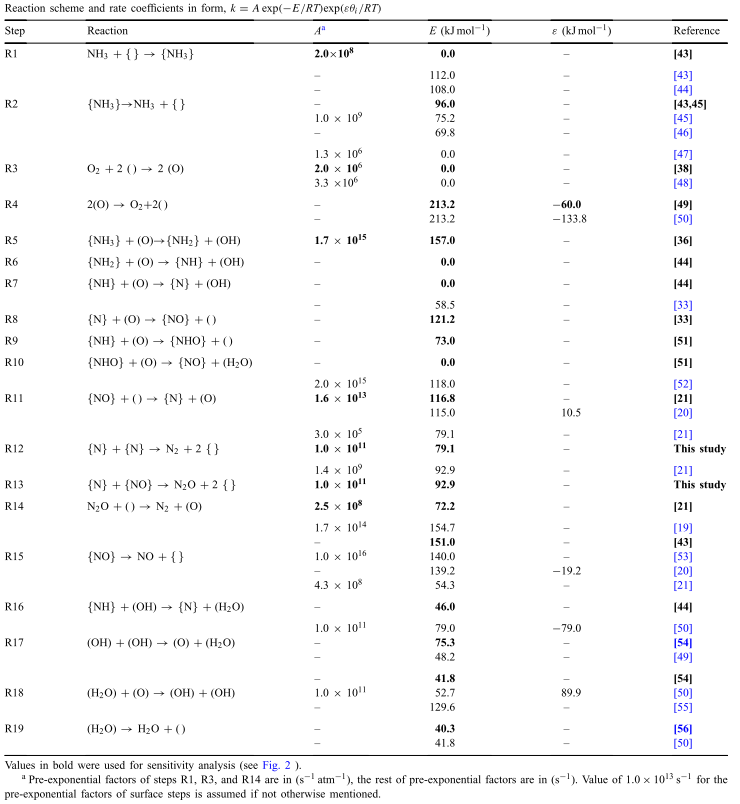
\includegraphics[width=\textwidth]{ammonia/ReactionScheme.png}
    \caption{\cite{Rebrov2002}}
    \label{fig:my_label}
\end{figure}

Relation to nanoparticle size
It was also reported that the stoichiometry of oxygen chemisorption increases by a factor 2.7 with increasing platinum crystallite size. This could also lead to an increase of the reaction rate if the oxygen adsorption is the rate-determining step in this system.

\subsection{Particle-Size Effect in Catalytic Oxidation Over Pt Nanoparticles}

Alexandr Yu. Stakheev, ..., Valerii I. Bukhtiyarov, in Advanced Nanomaterials for Catalysis and Energy, 2019

Relationships between turnover frequency and the size of supported Pt clusters are discussed for oxidation of hydrocarbons, CO, and NO by molecular oxygen. Analysis of the experimental data indicates that TOF tends to increase for bigger platinum particles. This tendency is particularly pronounced for the nanoparticles smaller than 4–5 nm. According to the most realistic models, the observed tendency stems from the deactivation of edge, corner, and neighboring atoms by two processes: (1) strong oxygen adsorption on edge and corner atoms with high degree of coordinative unsaturation, and (2) oxidation of Pt to PtOx, which is facilitated over undercoordinated sites. As the metal clusters grow in size, the fraction of undercoordinated edge and corner atoms decreases leading to the increase in experimentally observed TOF.


The increase of supported platinum particle size led also
to considerable changes in selectivity in the ammonia oxidation over a Pt/Al2O3 catalyst [7,22,26]. Large crystallites of 15.5 nm, for which over 98\% of the surface atoms are plane atoms [28], exhibited low selectivity to nitrogen formation. Selectivity to nitrogen increased with decreasing platinum loading

\subsection{Stability}

The turnover frequency TOF quantifies the specific activity of a catalytic centre for a special reaction under defined reaction conditions by the number of molecular reactions or catalytic cycles occurring at the centre per unit time. For heterogeneous catalysts the number of active centres is derived usually from sorption methods.

Separate from the TOF, evaluating the catalytic activity, the turnover number (TON) value is an important parameter to evaluate the stability of the catalyst. In homogeneous and heterogeneous catalysis, the TON is a dimensionless number,24,25 which is defined as the number of the molecules produced per catalytic site before deactivation under given reaction conditions. That is to say, the catalyst can achieve the total number of turnovers until it is totally dead, regardless of the reaction time.26 In this respect, an ideal catalyst should have an infinite TON. Thus, the TON represents the maximum yield of products attained from an active catalytic site up to the decay of activity for a specific reaction. The TON of a catalyst for water oxidation is calculated according to Eq. (5):


\subsection{Linking strain and reactivity}

Hammer and Noskrov blabla

    \section{X-ray interaction with matter}

\subsection{Scattering from electrons and atoms}

We begin our discussion of x-ray scattering by first considering scattering from a single free electron using classical electromagnetic theory. During elastic scattering, the oscillating electric field of the x-ray wave exerts forces ($\vec{F} = q \vec{E_i}$ , $q$ represents the charge) on the electron, causing it to accelerate and oscillate in the same direction as the incident field.

The oscillating electron then emits a spherical wave with the same wavelength as the incident beam (Thomson scattering) and this is the scattered field.

If we consider how the incident x-ray wave will interact with the different charge elements relative to the origin of the atom, you can see from Figure 1.4 that there is a path length difference of   where  =  is the scattering vector and is equal to the change experienced by the wavevector during scattering.

\subsection{Diffraction}



\lipsum


\subsection{Reciprocal space}



\lipsum


\subsection{Brillouin zone}

The importance of the Brillouin zone stems from the description of waves in a periodic medium given by Bloch's theorem, in which it is found that the solutions can be completely characterized by their behavior in a single Brillouin zone.

The first Brillouin zone is the locus of points in reciprocal space that are closer to the origin of the reciprocal lattice than they are to any other reciprocal lattice points (see the derivation of the Wigner–Seitz cell). Another definition is as the set of points in k-space that can be reached from the origin without crossing any Bragg plane.

A related concept is that of the irreducible Brillouin zone, which is the first Brillouin zone reduced by all of the symmetries in the point group of the lattice (point group of the crystal).

k-vectors exceeding the first Brillouin zone (red) do not Brillouin any more information than their counterparts (black) in the first Brillouin zone. k at the Brillouin zone edge is the spatial Nyquist frequency of waves in the lattice, because it corresponds to a half-wavelength equal to the inter-atomic lattice spacing a.



    \section{SXRD}

\subsection{Crystal truncation rods}

Thus the diffraction intensity of the finite-sized crystal has diffuse streaks connecting all the Bragg points. The diffuse intensity far from the nodes is of order of magnitude $N^4$ compared with $N^6$ at the nodes.

Scattering that is sharp in two directions and diffuse in the third (referred to as a "rod" of scattering) must arise from a crystalline object that is localized in one dimension and extended in the other two.

We are then left with only the sixth component due to the sharply truncated surface. We will call these features "crystal truncation rods. '

We now wish to estimate the strength of the truncation rods in the Bragg geometry. We must first modify Eqs. (1) and (2) by including the x-ray coherence length, $m$ (measured in unit cells), of the experimental configuration. This broadens all the diffraction features to $\frac{1}{m}$ reciprocal units. The Bragg points then have intensity of order $N_1 N_2 N_3 m^3$, while the diffuse intensity is $N_1 N_2 m^2$

A typical penetration depth is $1 \mu m$ so $N_3 =10^3$ unit cells (perpendicular to the face). With $m \approx 100$ unit cells, this gives a relative intensity
$\frac{I(Bragg peak)}{I(truncation rod)} = N_3 m \approx 10^5$

More roughness means wider Bragg peaks and deeper valleys between the BP.

It is not clear that different detailed models of roughness could be distinguished at this level of accuracy. One central concept to all descriptions of crystal truncation rods, however, is the continuation of the crystal lattice into the roughened region (not defects, keeping symmetry).

\subsection{Reciprocal space mapping}


\lipsum


\subsection{Reflectively}


\lipsum


\subsection{Computer programs}


\lipsum


\subsubsection{RefNX}


\lipsum


\subsubsection{ROD}

\lipsum


    \section{BCDI}

\subsection{Coherent diffraction}

Bragg coherent diffractive imaging (BCDI) is a lensless x-ray imaging technique that uses computational algorithms in place of physical lenses to achieve high-resolution imaging. It can be used to visualize the Bragg electron density and atomic displacement fields of crystalline materials in three-dimensional (3D) detail and with nanometer resolution.

We focus only on elastic scattering as that is the main process exploited when studying the structure of materials (the x-ray photon is elastically scattered (energy is conserved) and both the incident and scattered photons have the same wavelength).

By adding up the scattered amplitudes of an arrangement of atoms, we can then get the diffracted amplitude for a crystal. Note that the following derivations only apply if the diffraction pattern is viewed at a distance far away from the diffracting object. This region is known as the far-field or Fraunhofer region.

\subsection{Phase retrieval}

Basic algorithm is Error-Retrieval (ER), quick but can converge towards local minimum. 
The support corresponds to a shape when the object is included. The density of the object is thus equal to zero outside the support. (Fienup, 1978).

In practice, a slow convergence of the ER algorithm is often observed. The error-metric does not evolve and the algorithm is sort of stuck in a local minimum.

To overcome the problem of stagnation in local minima from ER, (FIenup, 1982) introduced the Hybrid-Input-Output algorithm, that differs in its application of real space constraints. Feedback parameter $\beta$, 
In practice, this adaptation is efficient and significantly enhances the convergence speed. It can be seen as a little perturbation that allows to leave a local minimum.


However, the HIO algorithm still fails sometimes, and this explains why the ER and HIO algorithms are generally used in combination.

\subsubsection{Support determination}
There are several techniques to estimate the support. In some cases, the shape and dimensions of the object have been already determined by other techniques (such as SEM or AFM for instance), and a support can be built from this knowledge. 

\subsubsection{Patterson function}
When the shape of the object is unknown, a rough estimate of the support can be obtained from the diffraction signal using the autocorrelation function (Marchesini 2003). It is based on the Patterson function which can be defined as the invert Fourier transform of the diffracted intensity. This function can be expressed as the convolution of the complex electron density.

The size of the crystal is overestimated by the Patterson function, since it provides its autocorrelation. In practice, a non uniform density leads to a non-trivial shape of the autocorrelation. The function needs to be threshold to start with a reasonable approximation. In most of the reconstructions in this manuscript, the threshold was set to 2\% of the maximum of the Patterson function. As discussed by Vaxelaire (2011), the method is not adapted to highly strained objects.


For large strain, the diffraction pattern has a large extent in the reciprocal space
(Beutier et al. 2013a). As a consequence, the Patterson function underestimates the size of the object, preventing any chance of success in the phase-retrieval procedure. In summary, if the shape and size of the object is unknown, it is not recommended to use the autocorrelation function as a first estimate of the support in the case of an highly strained system.

In combination of the ER and HIO algorithms, a third algorithm is routinely used for CDI. It is known as the shrink wrap (SW) algorithm and allows to update the support during the reconstruction. It was first introduced by Marchesini (2003) and has proven to greatly improve the convergence of the procedure.

In practice, the estimate is smoothed by convolution with a Gaussian. After convolution, a thresholding is applied to the smoothed image to a typical value of 10\% of the maximum value of the amplitude. Values above the threshold are set to 1 and values below are set to 0. The threshold is generally set to such low values to avoid to suppress too large parts of the support. Nevertheless, the convolution step allows to recover from a support that has been reduced

\subsection{Accessing strain and displacement}


\lipsum


\subsection{Computer programs}

\subsubsection{\textit{PyNX}}
Coherent X-ray imaging techniques developed during the last 20 years thanks to high brilliance in synchrotrons. Wide range of techniques:

\begin{itemize}
    \item Phase Contrast Imaging
    \item Coherent Diffraction Imaging, allowing to reconstruct single objects from their diffraction pattern alone, including strain imaging of crystalline nano-objects in the Bragg geometry.
    \item X-ray Ptychography, used in both near and far field regime, developed for imaging extended objects (larger than the incident beam), both in small angle and Bragg geometry, also usable in the Fourier regime by scanning the transmitted beam.
\end{itemize}
These techniques all provide high resolution 2D or 3D imaging, down to 5 to 15 nm resolution, depending on the instrumental setup.

Requires a coherent X-ray beam, readily available at synchrotrons facilities. Will benefit from upgrades of synchrotrons rings, which promises 2 orders of magnitude increase in the available coherent X-ray flux thanks to higher brilliance. This will enable faster dynamics and imaging experiments as well as reaching higher resolutions.
Higher energy coherent X-ray ($\>20 keV$) will enable data collection for thicker samples and allow to mitigate radiation damage with lower absorption.

PyNX has open-source coherent X-ray imaging modules \parencite{Favre-Nicolin2020}. All calculations for coherent imaging modules (\texttt{cdi, ptycho, wavefront}), respectively for Coherent Diffraction Imaging, Ptychography and coherent wavefront propagation (mostly used for simulation purposes) are executed on the GPU by using pyCUDA or pyOpenCL libraries. Language and GPU automatically selected based on tests.

Autocorrelation

The CDI technique consists of reconstructing an object from a far-field diffraction pattern alone, a technique which has been expanded to 3D reconstruction by collecting multiple ($>100$) projections around a rotation axis, either in the small angle, or in the Bragg geometries - the latter approach yielding information about strain in the reconstructed object \parencite{Li2020}.

In order to recover the object from non-redundant diffraction data, it is necessary to recover the lost phases of the measured amplitude (c.f. phase loss problem).

A variety of algorithms are available, all of which rely on alternating between a real-space estimate of the object and diffraction (Fourier) space, where an amplitude constraint can be applied from the measured intensity.


\subsubsection{\textit{bcdi}}

\subsubsection{Preprocessing}

Signal to noise ratio that influence FFT window size for cropping

Oversampling ratio

Poisson (Shot) noise 

\subsubsection{Postprocessing}

This section tries to detail the postprocessing of the phase and amplitude following the phase retrieval.

The 3D diffraction pattern is centered on its center of mass, and cropped to fit the FTT requirements. Its center is the center of the FFT array, which becomes the center of the reconstructed object. Phase and displacement can be inverted ??

\begin{minted}{python}
if invert_phase:
    phase_fieldname = "disp"
else:
    phase_fieldname = "phase"
\end{minted}

The shape of the object that is post processed is determined by a threshold, here 0.05, with a 10 padding.
\begin{minted}{python}
nz, ny, nx = obj.shape

zrange, yrange, xrange = pu.find_datarange(
	array=obj, amplitude_threshold=0.05, keep_size=prm.get("keep_size", False)
)

numz = zrange * 2
numy = yrange * 2
numx = xrange * 2
\end{minted}

\begin{figure}[ht]
    \centering
    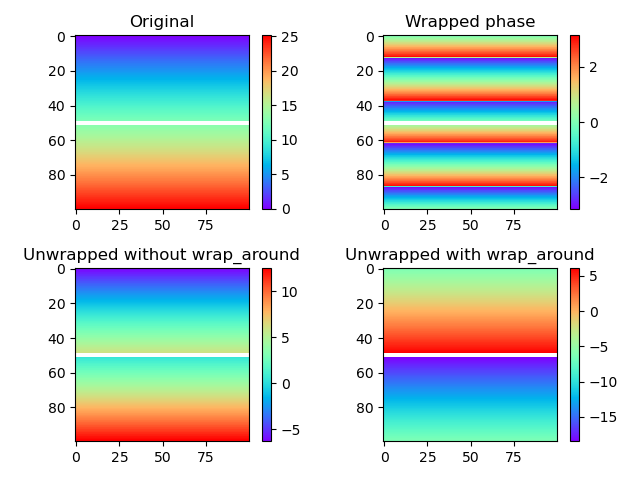
\includegraphics[width=\textwidth]{Images/phase_unwrapping.png}
    \caption{Phase unwrapping with skimage package.}
    \label{fig:phase_unwrap_skimage}
\end{figure}

Firstly, the phase outside a certain threshold (default value 0.05) is set to zero. A different threshold, lower than the isosurface threshold, is used on the amplitude to compute the support so that surface voxels aren't accidentally excluded from the correction.
The phase is then unwrapped, thanks to the skimage method (see figure \ref{fig:phase_unwrap_skimage}). It is then wrapped properly between the maximum and minimum of the phase.

\begin{minted}{python}
    phase, extent_phase = pu.unwrap(
        avg_obj,
        support_threshold=threshold_unwrap_refraction,
        debugging=debug,
        reciprocal_space=False,
        is_orthogonal=is_orthogonal,
    )
    
    extent_phase = phase.max() - phase.min()
    
    phase = (obj - start_angle + range_angle) \% range_angle + start_angle
\end{minted}

Secondly, the phase ramp is removed before phase filtering. To do so, the gradient of the phase is computed in three directions. It returns a set of ndarrays corresponding to the derivatives of the phase with respect to each dimension. Each derivative has the same shape as f.
The points for which the gradient is higher than the threshold ($\approx 1$) are ignored. The mean of the other points is returned as the ramp along that direction.

\begin{minted}{python}
    # Detail below
    amp, phase, rampz, rampy, rampx = pu.remove_ramp(
        amp=abs(avg_obj),
        phase=phase,
        initial_shape=original_size,
        method="gradient",
        amplitude_threshold=isosurface_strain,
        threshold_gradient=threshold_gradient,
    )
    
    # Define the support from the amplitude
    support = np.where(amp > amplitude_threshold * abs(amp).max(), 
                        1, 0)
    
    # Compute gradient
    gradz, grady, gradx = np.gradient(phase, 1)
    
    # Remove points lower than threshold
    threshold_gradient = 1.0
    supportz = np.where(abs(gradz) < threshold_gradient, 1, 0)
    
    # Make sure there  are no points outside the support
    supportz = supportz * support
    
    # Ramp is the mean value
    rampz = gradz[supportz == 1].mean()
    
    # Create mesh grid
    myz, myy, myx = np.meshgrid(
        np.arange(0, nbz, 1),
        np.arange(0, nby, 1),
        np.arange(0, nbx, 1),
        indexing="ij",
    )
    
    # Remove phase gradient
    phase = phase - myz * myrampz - myy * myrampy - myx * myrampx
\end{minted}

Example of gradient computation in python, using the nearest neighbours, see example applied to object phase in figure \ref{fig:phase_grad}.
\begin{minted}{python}
    f = np.array([1, 2, 4, 7, 11, 16], dtype=float)
    np.gradient(f) = array([1. , 1.5, 2.5, 3.5, 4.5, 5. ])
\end{minted}

\begin{figure}
    \centering
    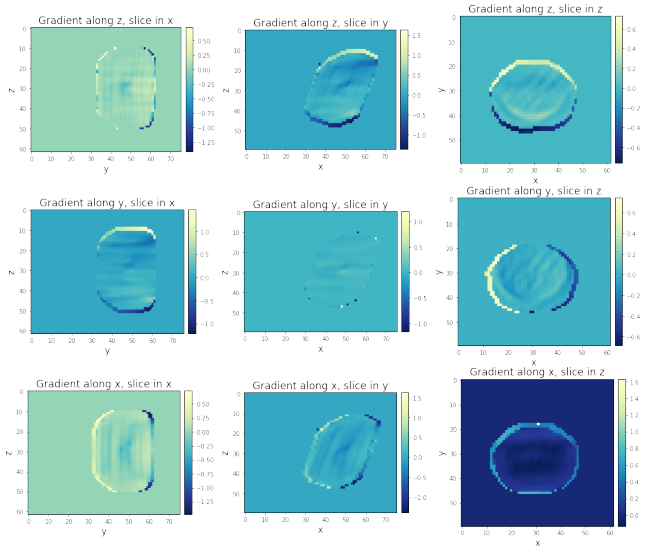
\includegraphics[width=\textwidth]{Images/phase_grad.png}
    \caption{Phase gradients}
    \label{fig:phase_grad}
\end{figure}

Thirdly, the phase offset is removed. Careful here, the threshold used is \verb|isosurface_strain|, the offset is either the value at the COM of the amplitude, or the mean value of the phase.

\begin{minted}{python}
    # Phase offset removal, detail below
    support = np.where(amp > isosurface_strain * amp.max(), 1, 0)
    phase = pu.remove_offset(
        array=phase,
        support=support,
        offset_method=offset_method, # usually mean, or COM
        phase_offset=phase_offset, # usually 0
        offset_origin=offset_origin, # usually not pre-determined
        title="Phase",
        debugging=debug,
    )
    
    # COM
    if offset_method == "com":
        zcom, ycom, xcom = center_of_mass(support)
        array = array - array[zcom, ycom, xcom] + phase_offset
    # mean
    elif offset_method == "mean":
        array = array - array[support == 1].mean() + phase_offset
        
     # wrap again
     phase = (phase - start_angle + range_angle) \% range_angle + start_angle
\end{minted}

Once that the phase is unwrapped, and that the phase ramp and offset are removed, the phase is averaged over a window and apodized to reduce noise in strain plots. The phase is averaged using a kernel of half-width \verb|half_width_avg_phase|. For the apodization, the diffraction pattern is recomputed with \verb|numpy.fft.fftn()|. This function computes the N-dimensional discrete Fourier Transform over any number of axes in an M-dimensional array by means of the Fast Fourier Transform (FFT). The zero-frequency component is shifted to the center of the spectrum using \verb|numpy.fft.fftshift()|.
An apodization window 

\begin{minted}{python}
    # compute support
    support = np.where(amp < isosurface_strain, 1, 0)
    
    # Average phase with nearest neighbours
    phase = pu.mean_filter(
        array=phase, support=support, 
        half_width=half_width_avg_phase, # usually 1
    
    # Apodization
    amp, phase = pu.apodize(
        amp=amp,
        phase=phase,
        initial_shape=original_size,
        window_type=prm.get("apodization_window", "blackman"),
        sigma=prm.get("apodization_sigma", [0.30, 0.30, 0.30]),
        mu=prm.get("apodization_mu", [0.0, 0.0, 0.0]),
        alpha=prm.get("apodization_alpha", [1.0, 1.0, 1.0]),
        is_orthogonal=is_orthogonal,
    )
    
    # Compute electronic density
    avg_obj = amp * np.exp(1j * phase)
\end{minted}
    
The phase is now corrected. The following steps are the centering of the object, as well as the interpolation of the arrays in the orthogonal reference frame where $\vec{q_{com}}$ is aligned onto the reference axis.
\begin{minted}{python}
    # Centering of array
    if centering_method == "max":
        avg_obj = pu.center_max(avg_obj)
        # shift based on max value,
        # required if it spans across the edge of the array before COM
    elif centering_method == "com":
        avg_obj = pu.center_com(avg_obj)
    elif centering_method == "max_com":
        avg_obj = pu.center_max(avg_obj)
        avg_obj = pu.center_com(avg_obj)
        
    # Calculate q of the Bragg peak in the laboratory frame
    q_lab = (
        setup.q_laboratory
    )  # (1/A), in the laboratory frame z downstream, y vertical, x outboard
    qnorm = np.linalg.norm(q_lab)
    q_lab = q_lab / qnorm
    
    # Find Bragg peak
    bragg_peak = bu.find_bragg(
        data=data,
        peak_method="maxcom",
        roi=detector.roi,
        binning=None,
    )
    
    # Compute atomic planar distance
    planar_dist = 2 * np.pi / qnorm  # qnorm should be in angstroms
    planar_dist = planar_dist / 10  # switch to nm
        
    # Find inplane and outofplane angles from setup
    # and Bragg peak
    setup.correct_detector_angles(bragg_peak_position=bragg_peak)
    prm["outofplane_angle"] = setup.outofplane_angle
    prm["inplane_angle"] = setup.inplane_angle
        
    # Orthogonalise object
    obj_ortho, voxel_size, transfer_matrix = setup.ortho_directspace(
        arrays=avg_obj,
        q_com=np.array([q_lab[2], q_lab[1], q_lab[0]]),
        initial_shape=original_size,
        voxel_size=fix_voxel,
        reference_axis=axis_to_array_xyz[ref_axis_q],
        fill_value=0,
        debugging=True,
        title="amplitude",
    )
\end{minted}

The orthogonalised object is re-centered on its center of mass, the phase unwrapping, the phase ramp removal and the phase offset removal are repeated. To resume, \verb|threshold_unwrap_refraction| is only used for the phase unwrapping, whereas  \verb|isosurface_strain| is used for both the phase ramp removal and the phase offset removal.
In order to facilitate the analysis of data-sets collected on the same object, the values of these two parameters should be the same as much as possible. In any case, they should be kept in mind when analysing the data.
Do not forget the -1 sign in the phase if the phasing algorithm is python or matlab-based.
Finally, the strain is computed from the phase.

\begin{minted}{python}
    # Add offsets if defects
    if method == "defect":
        offsets = 2 * np.pi / 10 * np.linspace(-10, 10, num=11)
    else:
        offsets = (0,)
        
    for offset in offsets:
        # offset the phase
        if method == "defect":
            temp_phase = np.copy(phase)
            temp_phase = temp_phase + offset
            # wrap again the offseted phase
            temp_phase = util.wrap(
                obj=temp_phase,
                start_angle=-extent_phase / 2,
                range_angle=extent_phase
            )
        else:  # no need to copy the phase, offset = 0
            temp_phase = phase

        # calculate the strain for this offset,
        # disp = planar_distance / (2 * np.pi) * temp_phase,
        if reference_axis == "x":
            _, _, temp_strain = np.gradient(
                planar_distance / (2 * np.pi) * temp_phase,
                voxel_size[2],
            )  # q is along x after rotating the crystal
        elif reference_axis == "y":
            _, temp_strain, _ = np.gradient(
                planar_distance / (2 * np.pi) * temp_phase,
                voxel_size[1],
            )  # q is along y after rotating the crystal
        else:  # "z"
            temp_strain, _, _ = np.gradient(
                planar_distance / (2 * np.pi) * temp_phase,
                voxel_size[0],
            )  # q is along z after rotating the crystal

        # update the strain values
        strain = np.where(abs(strain) < abs(temp_strain), strain, temp_strain)
\end{minted}


\subsubsection{\textit{Gwaihir}}
    \section{XPS}

\subsection{Spectroscopy}

\subsection{Peak shape}

Read thesis on XPS
    \section{SixS beamline}

Presentation of the MED environment ... 

\subsection{Mass flow controller}

\subsection{Residual Gas Analyser}

\subsection{Diffractometer}

Horizontal or vertical setup.
    
% Results
    \chapter{Results}
    \textcolor{red}{This Chapter should demonstrate that you have conducted a thorough and critical investigation of relevant sources.
Apart from a presentation of the sources of your data, this chapter allows you to critically discuss the data (whatever these data are, ‘quantitative’ or ‘qualitative’, primary or secondary), which is proof of good research. You can even do good research with poor data but you must demonstrate that you are aware of the data quality and accordingly are careful in your interpretations. Essentially, there are three aspects to consider:
\begin{enumerate}
\item	Reliability, which, for example, could depend on whether they are estimates or more direct evidence;
\item	Representativity, which is about how typical the data are; for example, you may have arguments why the very few cases are typical or you may carry out statistical tests;
\item Validity, which is about the relevance of the data for your case. Strictly speaking, sometimes no valid data are available but one may argue that there are other data which could be used as ‘proxies’.) 
\end{enumerate}
}

\section{Operando and in-situ experiments at SixS}



\section{BCDI on isolated Pt nanoparticles}

\textbf{Here, we will evaluate the metal-support interaction during reaction by monitoring the activity and structure evolution of the Pt NPs dewetted on three different support materials: sapphire, MgO and TiO2 [6]. This will allow examining the effect of the support on the metal catalyst. A careful in situ analysis of the properties of the nanoparticles (size, shape, strain, refaceting, support interaction, etc) in 3D is of essential importance to gain more understanding of the behaviour of these nanocrystals during a catalytic reaction.}

We want to evaluate the strain evolution of Pt particles and probe the impact of the support during CO oxidation.

\subsection{Preliminary test on gas reactor}

We performed several test on the small gas reactor to see how high we could go in temperature, which reactions happen at which temperature, etc ...
The data is in $PhDScripts/test\_reactor\_cell$

On 20/01, we confirmed that batch were usefull ?  (long batch stochio) and that products of both reactions (for the production of CO2, and then of nitrogen oxides respectively from CO and NH3 can be detected !)

Atmospheric pressure : $\approx$ 1 bar = 1 013.25 mbar = 1 013.25 hPa


uhv = 10 -9 mbar, 10-7 pascal

near ambient pressure ($>$ 1 mbar) 

DATA ACQUISITION

Rotating the sample results in rotating the reciprocal space
Whenever this happens, a diffracted beam is originated in the center of the Ewald sphere and passes through the reciprocal point that lies on the Ewald spherical surface... In these circumstances the so-called Bragg law is fulfilled. The set of all diffracted beams constitute the so-called diffraction pattern, which is subject to detection and evaluation. The reader should be aware that a complete diffraction pattern can contain a highly variable number of diffraction beams, from hundreds (simple inorganic compounds) to hundreds of thousands (proteins or viruses).
 
Ewald sphere is centered on the sample, reciprocal lattice on where $\vec{k_i}$ (from the sample) meets the sphere

Larger q -> higher hkl indexes

\subsection{Measurements}



\lipsum


\subsection{Reaction}


\lipsum



\section{SXRD on Pt 100 and Pt 111}
\subsection{Surface reconstruction}
\lipsum

\subsection{CTR and roughness}

\lipsum

\section{Ambient pressure XPS}
\subsection{Multi component analysis at ambient pressure}


    
    \section{Empirical Analysis}
    \section{Empirical Analysis}

\textcolor{red}{This chapter covers three areas: analysis of the data; discussion of the results of the analysis; and how your findings relate to the literature. The analysis of the data can be discussed here but the details of any analysis, such as statistical calculations, should be shown in the appendices. You should present any discussion clearly and logically and it should be relevant to your research questions/hypotheses or aims and objectives. Insert any tables or figures that you decide are important in a relevant part of the text not in the appendices, and discuss them fully. Make sure that you relate the findings of your primary research to your literature review. You can do this by comparison: discussing similarities and particularly differences. If you think your findings have confirmed some literature findings, say so and say why. If you think your findings are at variance with the literature, say so and say why.}

    
% Big data
    \chapter{Transitioning to big data at Synchrotrons}
    \section{Jupyter Notebook}
interface

\lipsum

\section{Standards for data reproducibility}

\lipsum
NXS, CXI, , reproducibility, repositories, PEP

    \section{Parallelism}

\lipsum

\section{Machine Learning}

\lipsum


    
% Conclusion
    \chapter{Conclusion}
    \section{Research aim and results}

This thesis was aimed at understanding, \textit{operando}, the evolution of catalysts surfaces during ammonia oxidation.
To do so, mainly three techniques have been used, Bragg coherent diffraction imaging, surface x-ray diffraction, and x-ray photoelectron spectroscopy, combined with mass spectrometry measurements.
These techniques are compatible with near-ambient pressure conditions, allowing to reduce the pressure gap in heterogeneous catalysis.
To bridge the material gap, large Pt nanoparticles and single crystals were used.
Throughout this work, low \ce{O_2}/\ce{NH_3} partial pressure ratios and temperatures were linked with selectivity towards \ce{N_2}, whereas high \ce{O_2}/\ce{NH_3} ratios and temperatures were linked to an increased selectivity towards \ce{NO} and \ce{N_2O}.
This is consistent with the reaction selectivity reported for industrial catalysts, which supports the use of nanoparticles and single crystals as model catalysts to improve the system understanding.

Pt nanoparticles epitaxied on sapphire were first measured at \qtylist{300;500;600}{\degreeCelsius} with SXRD during ammonia oxidation, starting with the introduction of ammonia in the reactor, and followed by a progressive increase of the oxygen pressure (\ce{O_2}/\ce{NH_3} = \{0, 0.5, 1, 2, 8\}).
The average shape of the Pt nanoparticles is mainly constituted of \{111\}, \{110\}, \{100\} and \{113\} facets.
A progressive reshaping of the nanoparticles was revealed at \qty{600}{\degreeCelsius} during reacting conditions.
Once \ce{O_2}/\ce{NH_3} = 1, and for increasing oxygen to ammonia ratios, the \{110\} and \{113\} facets surface coverage decreases, replaced by \{111\}, and \{100\} facets.

A single nanoparticle was then imaged with BCDI under inert atmosphere, at temperatures between \qtylist{25;600}{\degreeCelsius}.
A dislocation present at the interface from room temperature to \qty{125}{\degreeCelsius} was successfully removed by flash annealing above \qty{800}{\degreeCelsius}.
This dislocation was shown to have an impact of the thermal relaxation of the particle.
The \{111\} facets close to the interface evolve between \{211\}, \{221\} and \{110\} facets as a function of the sample temperature, and interfacial strain.
The introduction of ammonia in the reactor at \qty{600}{\degreeCelsius} resulted in a reversal of the facet strain, likely at the origin of the creation of an interfacial dislocation network, highlighting the link between facet and interfacial strain in nanoparticles.

Two additional nanoparticles were measured at \qtylist{300;400}{\degreeCelsius} during ammonia oxidation.
Different behaviours were revealed on the two nanoparticles, that exhibit a different size, shape, facet coverage, and initial strain state.
The surface of the larger nanoparticle (particle \textit{C}, \qty{800}{\nm} wide) is constituted by  \{111\}, \{110\}, and \{100\} facets.
Particle \textit{C} showed a reversible decrease/increase of homogeneous strain when ammonia was introduced/removed from the reactor, and could not be reconstructed without it.
A non-reversible increase in heterogeneous strain was measured at \qty{300}{\degreeCelsius} when first exposing the sample to reacting condition (\ce{O_2}/\ce{NH_3} = 0.5), no such increase was reproduced at the same conditions at \qty{400}{\degreeCelsius}.

The increase of homogeneous strain linked to the presence/absence of ammonia was not reproduced on the second nanoparticle (particle \textit{B}, \qty{300}{\nm} wide), and with \{113\} facets also present on its surface.
A non-reversible increase of heterogeneous strain was also measured at \qty{300}{\degreeCelsius}, but induced by the presence of ammonia, without oxygen.
The possibility of having an oxidised sample can explain this evolution under a reducing atmosphere, but is not observed for particle \textit{C}.
The appearance of a defect at \qty{400}{\degreeCelsius} was linked to a non-reversible and important increase of homogeneous strain during the oxidation of ammonia, which further increased as a function of the \ce{O_2}/\ce{NH_3} ratio.
This structural evolution is clearly visible in 3D, with volumes of missing Bragg electronic density.
The presence of defects could have a prominent role in the catalyst strain field and thus catalytic properties.
A global activation of the catalyst at \qtylist{300;400}{\degreeCelsius} was reported while the \ce{O_2}/\ce{NH_3} ratio was kept equal to 2, with an increased production of \ce{NO}, and in a lesser extent \ce{N2O}, at the detriment of \ce{N2}.

To better understand the role of each facet in the behaviour of the Pt nanoparticles, SXRD and XPS experiments were carried out at \qty{450}{\degreeCelsius} on Pt(111) and Pt(100) single crystals.
The samples were first exposed to high oxygen atmosphere (\qty{80}{\milli\bar}) to oxidise the Pt surfaces (total pressure always kept to \qty{500}{\milli\bar} by the use of argon for SXRD).
Two different oxygen to ammonia ratios are used after surface oxidation, by first introducing \qty{10}{\milli\bar} of ammonia (\ce{O_2}/\ce{NH_3} = \num{8}), and then reducing the oxygen pressure to \qty{5}{\milli\bar} (\ce{O_2}/\ce{NH_3} = \num{0.5}).
The XPS experiment was performed with the same ammonia to oxygen ratios, but at lower partial pressures (approximately \qty{10}{\percent} regarding the SXRD experiment).

The oxidation of both surfaces is first discussed.
Bulk \ce{Pt_3O_4} was identified on Pt(100), in a Pt(100)-($2\times2$) arrangement of mean thickness equal to \qty{16}{\angstrom} (\textit{i.e.} 3 unit cells thick).
Signals shifted in reciprocal space in comparison to the \ce{Pt_3O_4} peaks are also measured.
Both the \ce{Pt_3O_4} and shifted peaks were measured \qty{1}{\hour} after the introduction of oxygen, but could not be detected under a reduced oxygen atmosphere (\qty{5}{\milli\bar}), even after several hours.
Transient signals are measured instead, underlying the importance of the oxygen pressure in the surface oxidation.
Bulk \ce{Pt3O4} was not observed on Pt(111).
Nevertheless, a Pt(111)-($8\times8$) commensurate superstructure was clearly identified after \qty{9}{\hour}\qty{30}{\minute} of elapsed time under high oxygen atmosphere, and after \qty{23}{\hour}\qty{30}{\minute} under reduced oxygen atmosphere.
From the intensity distribution of the related out-of-plane signals, this structure was determined to be a few layers thick.
Additional in-plane signals are also detected as soon as oxygen is introduced in the reactor, at both pressures, linked to a Pt(111)-($6\times6$)-R\ang{\pm 8.8} structure.
The intensity of those signals decreases once the Pt(111)-($8\times8$) structure is present, which supports a precursor link between both structures.
% Moreover, when describing the signals with the Pt(111)-p$\begin{pmatrix} 1.08 & -0.21 \\ -0.21 & 1.08 \end{pmatrix}$ matrix, which results in a real space angle of \ang{137.4}, a second-order signal is shared.
Signals measured in the XPS O 1s level at reduced oxygen atmosphere and attributed to surface oxygen species are more important for Pt(100) than Pt(111), showing that Pt(100) surface is more readily oxidised than Pt(111).
Oxidation of Pt(111) and Pt(100) was linked to increased surface roughness, and to compressive out-of-plane strain with respect to inert atmosphere for Pt(111).

Different behaviours were measured on both surfaces during reacting conditions.
Under high \ce{O_2}/\ce{NH_3} ratio, which favours the production of \ce{NO}, surface oxides are directly removed from Pt(111), but reconstruct with a (10x10) arrangement on Pt(100).
Oxygen species signals in the O 1s level are weak for Pt(111), difficult to dissociate from the background, whereas peaks are clearly detected for Pt(100).
The difference in surface oxygen presence is already observed during previous surface oxidation.
The reconstruction of the Pt(100) surface is linked to the persisting presence of surface oxygen species during ammonia oxidation, thereby differing from the Pt(111) surface.
Moreover, the selectivity towards \ce{NO} is increased for Pt(100), also linked to the more importance presence of surface oxygen, which is crucial in the production of \ce{NO} during the reaction mechanism \parencite{NovellLeruth2005, Offermans2006, Offermans2007, Imbihl2007, NovellLeruth2008}.
Increased roughness is also observed during this condition for both surfaces.

Pt(111) and Pt(100) show a similar selectivity towards \ce{N_2} when lowering the \ce{O_2}/\ce{NH_3} ratio to \num{0.5}.
The magnitude of the out-of-plane strain (surface relaxation), and the surface roughness, are already reduced in this condition for Pt(111), but stay at similar values for Pt(100).
On both surfaces, oxygen species are absent from the O 1s level, and adsorbed atomic nitrogen is measured, linked to the Pt(100)-Hex surface superstructure for Pt(100).
Adsorbed ammonia is also observed on Pt(111).

The difference in out-of-plane strain (surface relaxation) when lowering the \ce{O2}/\ce{NH3} ratio from \num{8} to \num{0.5} is in the same order of magnitude, but of different nature.
\qty{\approx 0.06}{\percent} tensile / compressive strain on Pt(100) /  Pt(111).
Most importantly, the strain is contained on the topmost layers of the platinum catalysts.
If one considers a Pt(100) surface voxel \qty{10}{\nm} thick, the corresponding averaged voxel strain would be equal to \qty{0.002}{\percent} with respect to the bulk lattice.
Therefore, the change of strain between reacting conditions becomes difficult to resolve, which can explain why no differences are observed on particle \textit{C} during ammonia oxidation.
Another factor to take into account is the increased surface roughness linked to high oxygen pressure, which has the effect of decreasing the intensity of the scattered photons far from the Bragg peak, and will thus reduce the experimental resolution.
Additional high-resolution studies could contribute to understanding the effect of adsorbates on surface relaxation.

The thesis demonstrates the importance of combining structural measurements at both the individual particle and particle assembly levels.
With Bragg coherent diffraction imaging (BCDI), we have demonstrated that depending on the morphology (shape, size, facet type and coverage, \textit{etc.}) and initial strain state of the Pt particles, different structural evolution are observed (in terms of strain, morphology, and defects) during the ammonia oxidation.
A better representation of the different behaviours followed by Pt particles during reaction, by measuring multiple individual particles, appears mandatory for a comprehensive understanding of the structure-activity relationship.
It is noteworthy that the strain at the particle/support interface seems to exert a pronounced influence on the particle behaviour.
Nanoparticles serve as a platform to explore the simultaneous structural evolution of diverse crystallographic facets at once.
Single crystal studies allow to better isolate the behaviours of single facets on nanoparticles.

\section{Perspectives}

This thesis has underlined the importance of bridging the material gap, by combining model catalysts with samples approaching the shape of industrial samples.
The structure evolution of Pt nanoparticles was shown to strongly depend on their size, shape, facet coverage and initial strain state.
The ammonia oxidation, which posses at least four different products, and a selectivity dependant on the reactant ratio, working temperature, and total pressure, draws a multi-dimensional parameter space only correctly addressed with information of different nature.

BCDI has proven to be powerful, but limited by the reconstruction process, as well as the time needed to find and image isolated nanoparticles.
Significant progress has already been made at the European synchrotron at the ID01 beamline, where rocking curves can be acquired under a minute.
\textit{Operando} measurements have proven to be challenging, Pt nanoparticles moving on the substrate at \qty{600}{\degreeCelsius} under reacting conditions, and sample environments failing during SXRD measurements.
Closing the pressure gap can be achieved for SXRD and BCDI by designing reactors resistant to highly oxidising atmosphere, and in this case, compatible with the ammonia/nitrogen oxide gas family, often banned due to their corrosive and toxic nature.
Future experiments must move towards industrial condition to be relevant, the importance of total pressure was demonstrated in this thesis with e.g. oxide formation on Pt(100) at \qty{80}{\milli\bar} and not at \qty{5}{\milli\bar}.
Simpler reaction cycles (e.g. by reducing the amount of \ce{O2}/\ce{NH3} ratios) will also help reduce the complexity of the data analysis.
A future reaction cycle is proposed.
First exposing the sample to increased oxygen pressure will reduce the time needed to detect potentially relevant oxides, as showcased here with the detection time of the Pt(111)-($8\times8$) structure, divided by \num{2.5} under \qty{80}{\milli\bar} of oxygen compared to \qty{5}{\milli\bar}.
A significant thickness of those platinum oxides could also be sufficient to be detected during BCDI experiments, especially now that the corresponding interplanar spacings are clearly determined.
Their impact of the facet strain in BCDI could then be determined by reconstructing the 3D strain tensor.
Higher oxygen pressure may reveal a role of platinum oxides during ammonia oxidation, invisible at lower pressure.
This will also remove the unknown regarding initial oxidised/contaminated states when introducing ammonia, and set a more systematic starting point for chemical cycles.
Ending the reaction cycle by having only ammonia in the reactor is also at the origin of large strain variations measured with SXRD, that could be more easily detected with BCDI.
In the future, surface x-ray experiments on Pt(110) and Pt(113) samples will add to our knowledge, and help better understand the structural behaviour of Pt nanoparticles.

Nevertheless, experimentally resolving the role of interfacial strain \textit{operando} could be performed by e.g. (i) exposing a nanoparticle that possesses an interfacial defect to reacting atmosphere, (ii) subsequently removing this defect by annealing, and (iii) repeating the exposition to reacting condition to observe a potential difference in the facet strain.
However, a certain control of the initial particle strain is needed.
The development of efficient simulation workflows to understand and de-correlate the effect of interfacial strain from adsorbant strain is also part of the solution.
The development of x-ray techniques that can bring higher statistics in the study of individual nanoparticles must be pushed forward.
In this perspective, x-ray Bragg ptychography is a technique that should receive increased interest since the measurement process can provide a unique solution.

The upgrade of synchrotrons is of key importance to efficiently navigate between different temperatures/pressures/reactant ratios.
For SXRD and BCDI, a reduced counting time will help catch transient structures, while increased photon count will increase the possibility to detect weak second and third order signals.
Moreover, BCDI gains from the increased coherent flux, while NAP-XPS also benefits from the increased photon flux.
Reaction cycles could also be repeated to increase the results significance, while changing the steps order.
Furthermore, a software upgrade is also needed, the surface x-ray diffraction community lacks an efficient and complete software combining data reduction and analysis.
For BCDI, the development of \textit{Gwaihir} was undertaken to respond to such needs from the community.
Additional work may address the data reduction automatisation by developing error-metrics for phase retrieval, methods to find the best solution, automatic facet detection in Python, \textit{etc}.
This would largely reduce the data reduction time, facilitating the analysis of multiple particles at various conditions.
A detailed study of the impact of trying to improve the image resolution by increasing the distance from the centre of the Bragg peak by combining simulations and experimental reconstructions would be of great interest to the community.
    
% Bibliography
    \phantomsection
    \printbibliography

% Appendices
    \appendix
    \chapter{(Appendix A)}
    \textcolor{red}{The final sections of your thesis are the appendices. Each appendix should be lettered (A, B, etc.,) and should consist of detailed information that is interesting but not essential to the main thrust of your findings section.\\
The appendices should be in the order that they are referred to in the main text. For instance, if Appendix A refers to something on page 25 and Appendix B refers to something on page 15, the appendices need to be re-lettered. This inconsistency occurs when text is moved around or inserted.)}


Gwaihir

Paper Ammonia

Paper MIR on strain and nano-twin ?

Paper Corentin on CO adsorption ?

    \input{Sections/6_Appendix/PythonScripts}

% 4ème de couverture
%%%%%%%%%%%%%%%%%%%%%%%%%%%%%%%%%%%%%%%%%%%%%%%%%%%%%%%%%%%%%%%
\Ifthispageodd{\newpage\thispagestyle{empty}\null\newpage}{}
\thispagestyle{empty}
\newgeometry{top=1.5cm, bottom=1.25cm, left=2cm, right=2cm}
\fontfamily{rm}\selectfont

\lhead{}
\rhead{}
\rfoot{}
\cfoot{}
\lfoot{}

\noindent 
%*****************************************************
%***** LOGO DE L'ED À CHANGER IMPÉRATIVEMENT *********
%*****************************************************
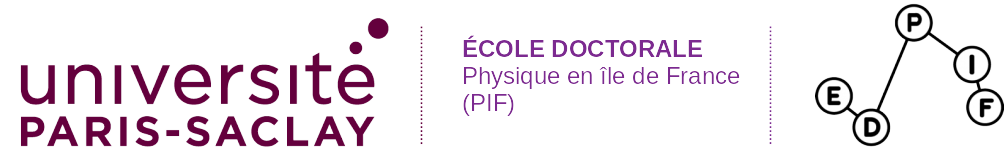
\includegraphics[height=2.4cm]{Images/logo_edpif_4eme.png}
\vspace{0.5cm}
%*****************************************************
\fontfamily{cmss}\fontseries{m}\selectfont

\small

\begin{mdframed}[linecolor=Prune,linewidth=1]

\textbf{Titre:} Propriétés catalytiques à l’échelle nanométrique sondées par diffraction des rayons X de surface et imagerie de diffraction cohérente

\noindent \textbf{Mots clés:} Diffraction, Catalyse, Surface, Structure, Déformation

\vspace{-.5cm}
\begin{multicols}{2}
\noindent \textbf{Résumé:} Le principal objectif est d'imager des nanostructures pour sonder les conditions in situ et operando ; mesurer la structure à l'échelle nanométrique et révéler également les effets de masse, de surface et d'interface ainsi que les défauts. Viser à terme à comprendre les phénomènes structurels importants pour les nanocatalyseurs et les relier à leur activité, sélectivité, réutilisabilité et durabilité. En complément des études cohérentes aux rayons X sur des particules individuelles, des techniques étudiants la moyenne des ensembles comme la diffraction des rayons X à incidence rasante seront employées pour voir si l'évolution des formes d'ensemble sont similaires à celles des nanoparticules uniques et sondent s'il y a une déconnexion entre les particules uniques et l'activité catalytique sur des billions de particules. La catalyse des nanomatériaux est apparue comme un moyen efficace d'exposer une surface plus élevée et d'accélérer les processus catalytiques en maximisant le rapport surface-volume. Le développement d'une catalyse hétérogène avec une sélectivité ciblant les 100\% est un défi constant ainsi que la compréhension de la durabilité et du vieillissement du catalyseur lui-même. Dans un procédé réel (réacteur d'usine de catalyseur, échappement de voiture, pile à combustible), l'évolution de la forme et de la déformation des nanoparticules catalytiques dans des conditions de réaction contribue au vieillissement du catalyseur et a un impact sur la durée de vie du dispositif. Cependant, le processus catalytique et les changements structurels associés restent encore mal compris. Comprendre comment la structure du catalyseur est affectée par la couche adsorbée dans des conditions de réaction est donc de la plus haute importance pour formuler des relations de performance de structure de catalyseur qui guident la conception de meilleurs catalyseurs.
\end{multicols}

\end{mdframed}

\begin{mdframed}[linecolor=Prune,linewidth=1]

\textbf{Title:}Catalytic properties at the nanoscale probed by surface X-ray diffraction and coherent diffraction imaging

\noindent \textbf{Keywords:} Diffraction, Catalysis, Surface, Structure, Strain

\begin{multicols}{2}
\noindent \textbf{Abstract:} The main objective is to image nanostructures to probe in situ and operando conditions; measure the structure at nanoscale and to reveal bulk, surface and interface effects, as well as defects. Ultimately aiming to understand the structural phenomena important for the working nanocatalysts and link them to their activity, selectivity, reusability and sustainability. In complement to coherent x-ray studies on individual particles, ensemble-averaging techniques like grazing incidence x-ray diffraction will be employed to see if the evolution of ensemble shapes is similar to the one of single nanoparticles and probe if there is a disconnect between single particles and the catalytic activity over trillions of particles. Catalysis of nanomaterials has emerged as an efficient way to expose higher surface area and accelerate catalytic processes by maximizing the surface-volume ratio. The development of heterogeneous catalysis with selectivity targeting the 100\% is a constant challenge as well as understanding the durability and ageing of the catalyst itself. In a real process (catalyst plant reactor, car exhaust, fuel cell) the shape and strain evolution of catalytic nanoparticles under reaction conditions contributes to the ageing of the catalyst and impact the lifetime of the device. However, the catalytic process and the associated structural changes remain poorly understood. Understanding how catalyst structure is affected by the adsorbed layer under reaction conditions is therefore of utmost importance to formulate catalyst structure performance relations that guide the design of better catalysts.
\end{multicols}
\end{mdframed}

%************************************
\vspace{\fill} % ALIGNER EN BAS DE PAGE
%************************************

\noindent
\color{Prune} \footnotesize Maison du doctorat, Université Paris-Saclay\\
2$^{\mathrm{e}}$ étage, aile ouest, École normale supérieure Paris-Saclay\\
4 avenue des Sciencs\\
91190 Gif-sur-Yvette, France
\end{document}

%%%%%%%%%%%%%%%%%%%%%%%%%%%%%%%%%%%%%%%%%%%%%%%%%%%%%%%%%%%%%%%%%%%%%%%%%%%%%%%%%%%%%%%%%%%%
